\documentclass[a4paper,11pt,twoside,openright]{book}							% COMANDI INIZIALI
\usepackage[italian]{babel}								% sillabazione italiana
\usepackage[utf8]{inputenc}								% Per le lettere accentate IN UNIX E IN WINDOWS
\usepackage{ragged2e}					 				% giustifica
\usepackage{amsmath}									% Per allineare le equazioni
\usepackage{amssymb}									% Per le lettere dell'indicatrice (mathbb)

\usepackage{graphicx}
\usepackage{amsthm}
\usepackage{amssymb}
\usepackage{amsmath}
\usepackage{mathtools}
\usepackage{caption}
\usepackage{booktabs}
\usepackage{hyperref}
\usepackage{float}
\usepackage{subfigure}


\justifying 										% giustifica

\date{28 Luglio 2014}
\author{Gabriele Mazza}
\title{Dimostrazione $S_{time}$ e $S_{space}$}

\begin{document}

%Indice e numerazione
\pagenumbering{arabic}

\chapter{Rifiuti nella provincia di Venezia}


L'applicazione scelta per il modello analizzato riguarda i dati di analisi di produzione di rifiuti urbani nel periodo di anni dal 1997 al 2011 nella provincia di Venezia. Per rifiuti urbani si intendono rifiuti domestici, prodotti in locali, aree pubbliche, parchi o giardini, spiagge o provenienti dalla pulizia delle strade o di altri luoghi pubblici. Non sono conteggiati i rifiuti speciali (tra cui ad esempio gli industriali, agricoli o provenienti da attività commerciali o di costruzione) o pericolosi (per i quali esistono programmi di smaltimento particolari).

I dati sono stati raccolti ed elaborati pubblicati dall'Agenzia regionale per la prevenzione e protezione ambientale del Veneto (Arpav) e sono disponibili sul sito di Open Data Veneto\footnote{\href{http://dati.veneto.it/dataset/produzione-annua-di-rifiuti-urbani-totale-e-pro-capite-1997-2011}{http://dati.veneto.it/dataset/produzione-annua-di-rifiuti-urbani-totale-e-pro-capite-1997-2011}} per la consultazione e il trattamento.

Per ogni comune della provincia di Venezia e per ogni anno è disponibile il numero di rifiuti totali raccolti in tonnellate e la popolazione residente. La popolazione è certamente un valore influente per la produzione di rifiuti, perciò la quantità di riferimento non sarà il valore dei rifiuti totali raccolti in ogni anno per comune, ma il valore pro capite.

Le coordinate spaziali dei comuni sono la longitudine e la latitudine, disponibili on line\footnote{\href{http://www.dossier.net/utilities/coordinate-geografiche/}{http://www.dossier.net/utilities/coordinate-geografiche/}}. Nel caso dei comuni con dato replicato (sez \ref{sez:comunireplicati}), sono state scaricate da Google Maps.


\section{L'inclusione dell'effetto del turismo}

Come è stato spiegato in precedenza, la produzione annua di rifiuti nei comuni può essere condizionata dalla popolazione. La parte residente è già stata inclusa nella risposta, poiché per uniformità i rifiuti sono espressi come valore pro capite nel comune. Tuttavia anche i turisti sono una componente non trascurabile di produzione di rifiuti urbani.

Nella provincia di Venezia sono presenti molte zone di elevata attrazione turistica. La più rilevante di queste è Venezia, ma si hanno anche zone balneari (come Lido di Venezia, Cavallino-Treporti, Jesolo, San Michele al Tagliamento, Bibione, ecc...). L'informazione scelta per sintetizzare l'attività turistica è il numero di posti letto totali del comune, valore disponibile grazie all'applicativo dell'Istat \textit{Atlante Statistico dei Comuni}\footnote{\href{http://www.istat.it/it/archivio/113712}{http://www.istat.it/it/archivio/113712}} per ogni anno. Il totale dei posti letto per comune è la somma di vari tipi di attività non solamente alberghiere (ad esempio sono conteggiati anche esercizi complementari, bed \& breakfast, campeggi) e saranno considerati normalizzati per la popolazione residente per uniformità con la risposta. I valori ricavati saranno inseriti nel modello come possibile covariata.


\section{Trattamento del dominio}

Per poter studiare il problema a livello computazionale occorre avere una buona approssimazione della frontiera della regione. Questa è disponibile nel pacchetto R \textit{raster} che descrive dati geografici di moltissime zone del mondo sia a livello nazionale che locale (nel caso italiano province e comuni) tramite poligoni molto precisi.

Una volta scaricata la provincia di Venezia si è riscontrato subito un problema di trattazione: la regione è composta da un insieme di 101 poligoni distinti (a causa delle numerose isole di cui è composta la laguna di Venezia) e ogni poligono ha un alto numero di vertici (ad esempio, la prima delle due regioni corrispondenti all'entroterra aveva 10538 vertici). Non è possibile analizzare il problema su un territorio così descritto, perciò è stata necessaria una analisi iniziale della frontiera per ridurne la complessità.

Oltre all'entroterra (composto da due poligoni) stati scelte solo le più importanti isole della laguna veneta: Venezia, Murano, Lido di Venezia e Pellestrina (più rilevanti a livello di popolazione e turismo). I poligoni sono stati semplificati in tutti i casi e uniti tra loro con ponti dove era possibile. Tra le isole collegate solamente via mare con il resto del territorio sono state simulati ponti in corrispondenza delle trafficate linee di trasporto pubblico con traghetto.

\subsection{Regression splines}

Per ridurre l'elevato numero di vertici di ognuno dei poligoni considerati si è scelto di ricorrere ad un'analisi di smoothing di dati funzionali. Ad ogni poligono è associata una coppia di funzioni: la latitudine e la longitudine rispetto all'ascissa curvilinea (disponibili per punti, corrispondenti ai vertici) che sono state rappresentate in basi e valutate in un mumero molto inferiore di punti, con i quali si è costruita la nuova definizione della regione.

Per avere una rappresentazione tramite funzioni di base di queste funzioni sono state provate più tecniche, ma la scelta definitiva è ricaduta sulle \textit{Regression Splines} cubiche senza penalizzazione della derivata seconda. Infatti i risultati non sono stati migliori negli altri casi a causa della zona interna alla laguna di Venezia, fortemente frastagliata: penalizzare la derivata seconda eliminava troppe asperità presenti sulle coste del territorio, mentre con \textit{Kernel Smoothing} sono state ricavate regioni che, dopo la triangolazione, presentavano troppi triangoli composti solamente da punti di frontiera (e quindi senza dati) rispetto agli altri metodi.

Una volta fissato un ragionevole numero di punti con cui descrivere la regione sono stati eseguiti più tentativi per decidere il miglior numero di basi necessario per l'analisi. Il criterio di scelta è stato complesso, poichè sono stati esclusi i valori che generavano intersezioni nella nuova descrizione della regione e comuni esterni alla frontiera. Ma la scelta del miglior numero di basi per \textit{Regression Splines} è ricaduta sul valore che, una volta eseguito lo smoothing della regione, causava la minor distanza tra i nuovi punti della regione e il poligono iniziale. In figura \ref{fig:Ven_ent1} è riportato il risultato dello smoothing sul primo poligono che descrive l'entroterra della provincia di Venezia (descritta con 100 punti, molto meno dei 10538 iniziali).  

\begin{figure}[!t]
\centering
\begin{minipage}{.32\textwidth}
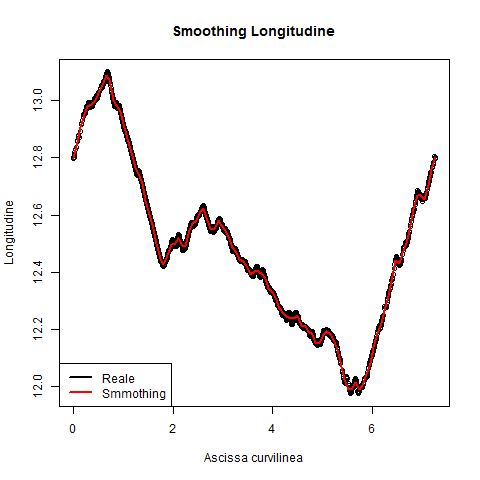
\includegraphics[width=\textwidth]{Immagini/Ven_Longitudine.png}
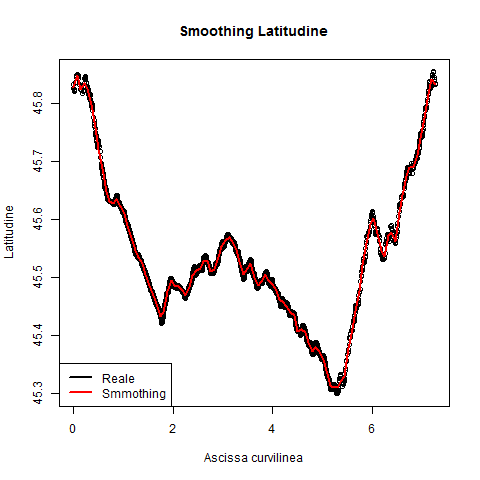
\includegraphics[width=\textwidth]{Immagini/Ven_Latitudine.png}
\end{minipage}%
\begin{minipage}{.64\textwidth}
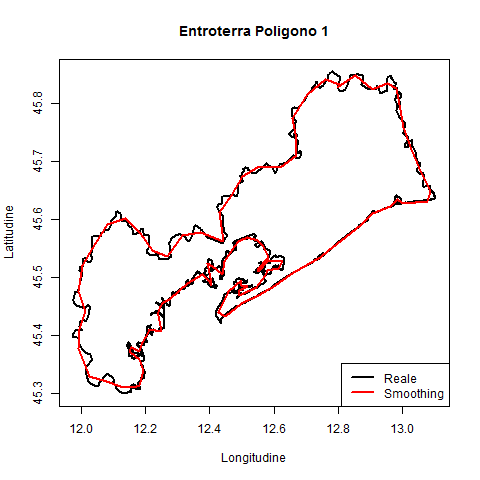
\includegraphics[width=\textwidth]{Immagini/Ven_Regione.png}
\end{minipage}
\caption{Smoothing con \textit{Regression Splines} cubiche per il primo poligono dell'entroterra della provincia di Venezia}
\label{fig:Ven_ent1}
\end{figure}

Dopo aver ripetuto l'analisi per ognuna delle isole scelte inizialmente la descrizione finale è stata ricavata unendo tra loro i nuovi poligoni. In seguito è stata eliminata una zona costiera dell'entroterra della laguna di Venezia che, sebbene sia presente sia in \textit{raster} che nei grafici di Google Maps, corrisponde ad una parte fangosa e paludosa e quindi disabitata. Non essendo possibile che su di essa siano prodotti rifiuti è stata tagliata dalla regione. Per questo motivo si troverà sempre una zona non analizzata sui grafici con mappe da Google Maps. In figura \ref{fig:Ven_rgm} è riportata la descrizione finale del dominio con i punti spaziali considerati (si consulti anche la sezione \ref{sez:comunireplicati}).
\begin{figure}[!t]
\centering
\subfigure[Provincia di Venezia]
   {
   \label{fig:Ven_rgm_tot}
	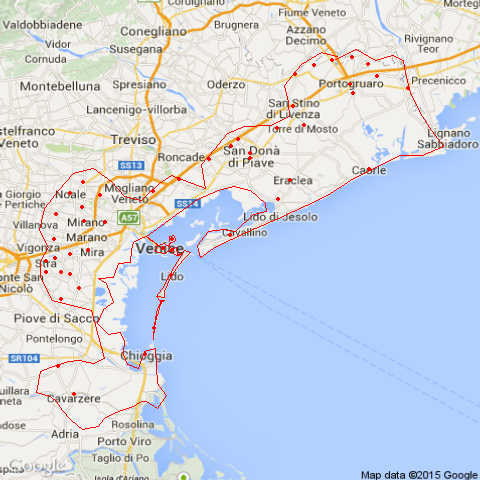
\includegraphics[width=0.46\textwidth]{Immagini/Ven_punti.png}   
   }
\subfigure[Zoom della laguna]
   {
   \label{fig:Ven_rgm_zoom}
	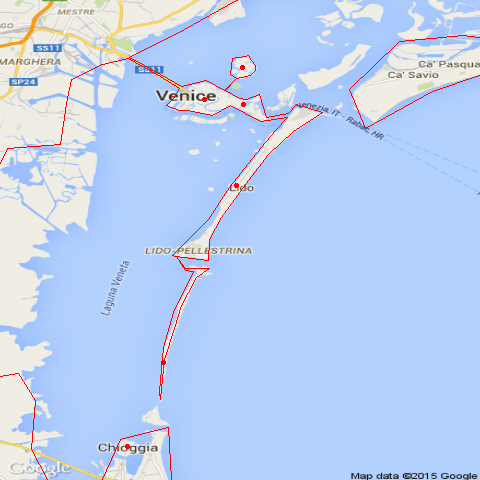
\includegraphics[width=0.46\textwidth]{Immagini/Ven_puntizoom.png}
   }
\caption{Frontiera e punti spaziali per la provincia di Venezia}
\label{fig:Ven_rgm}
\end{figure}

\subsection{Scelte particolari tra i comuni}
\label{sez:comunireplicati}

L'uso di valori pro capite per rifiuti e posti letto consente di replicare del comune anche su altri punti in cui risulta necessario. Ad esempio, le isole di Murano, Lido di Venezia e Pellestrina non sono sedi di comune, ma si riferiscono a Venezia. Quindi il dato di Venezia è stato replicato in queste isole ad ogni anno, per avere un valore di riferimento in quanto zone distaccate. Come si può notare in figura \ref{fig:Ven_rgm_zoom} anche nell'isola di Venezia è stato duplicato il dato, per avere una triangolazione  senza troppi triangoli composti solo da punti di frontiera in una zona della provincia di Venezia di particolare rilevanza.

Un caso particolare riguarda il comune di Cavallino-Treporti, che è stato istituito nel 1999 da una parte dei territori del comune di Venezia. La separazione all'interno dei dati, però, è presente dal 2002. Di conseguenza prima di questo anno il dato in Cavallino-Treporti è una replica del dato di Venezia.

\subsection{Triangolazione del dominio}

La triangolazione è stata prodotta tramite il pacchetto R \textit{RTriangle}. Poichè nella zona ad est i capoluoghi di comune sono meno fitti rispetto al resto della regione, è stata fissata un'area massima per i triangoli generati da \textit{RTriangle}. Questa scelta ha permesso di avere una descrizione del risultato più precisa nella zona balneare ad est, che come si potrà notare in seguito ha una grande importanza per la distribuzione dei rifiuti. Inoltre, il vincolo di area massima ha comportato la creazione di nuovi punti spaziali, che però restano senza dato per tutta l'analisi.

\begin{figure}[!t]
\centering
\subfigure[Provincia di Venezia]
   {
   \label{fig:Ven_rgm_tot}
	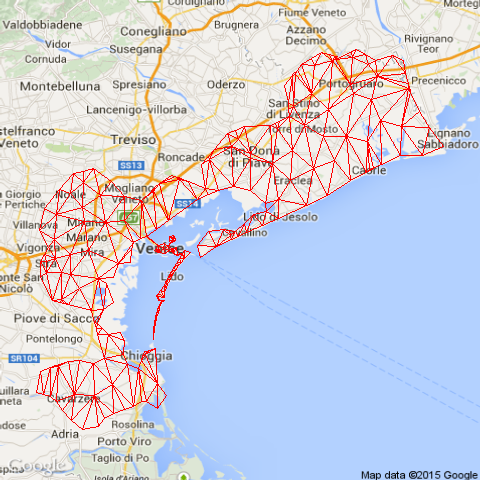
\includegraphics[width=0.46\textwidth]{Immagini/Ven_triang.png}   
   }
\subfigure[Zoom della laguna]
   {
   \label{fig:Ven_rgm_zoom}
	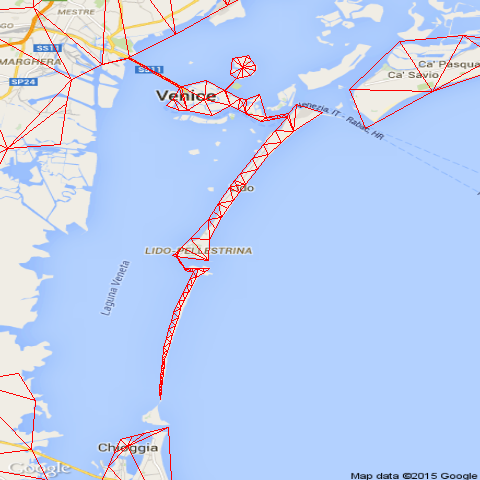
\includegraphics[width=0.46\textwidth]{Immagini/Ven_triangzoom.png}
   }
\caption{Triangolazione della provincia di Venezia}
\label{fig:Ven_rgm}
\end{figure}

In conclusione, il dominio è descritto da 414 punti (41 con dati, 373 di frontiera o aggiunti dalla triangolazione) e da 475 triangoli.


\section{Analisi senza covariate}
L'intervallo temporale per la descrizione del dominio è $[1997,2011]$, e i dati sono disponibili con cadenza annuale. Analogamente a quanto fatto per il dominio a forma di C, la prima cosa da fare è trovare dei buoni valori per $\lambda_S$ e $\lambda_T$ minimizzando la quantità $GCV(\underline \lambda)$ in (CITAZIONE NECESSARIA).

















\end{document}